\section{Implementation}

This section discusses the implementation of the Carat developer API prototype. The API aims to provide mobile application developers the ability to discover how a client mobile device's system settings and state affect the energy consumption of the device.

The design of such a service poses multiple challenges, as discussed in~\cite{7840871}. The dataset itself is large and incrementally changing as time passes, which makes static statistical analysis inconvenient. It is therefore practical to design the service in such a way that the analysis can be executed dynamically whenever the API is accessed. Another design challenge is to protect the privacy of the participants of the Carat project.

Association rules were selected as the basis of the API for two reasons. First, the association rules effectively hide all the details about individual Carat users protecting their privacy, while also enabling reasonably detailed view on how a devices system settings and state affect the energy consumption. Secondly, efficient parallel algorithms exist for generating association rules from huge datasets as discussed in detail in section \ref{association analysis}.

As discussed in~\cite{7840871}, the intention of the Carat API is to allow application developers to retrieve information about their application by authenticating with their developer key. The prototype described here, does not include authentication of application developers, but rather demonstrates the functionality that the API could offer provided that an authentication has been successfully completed. 

\begin{figure}[h]
	\centering
	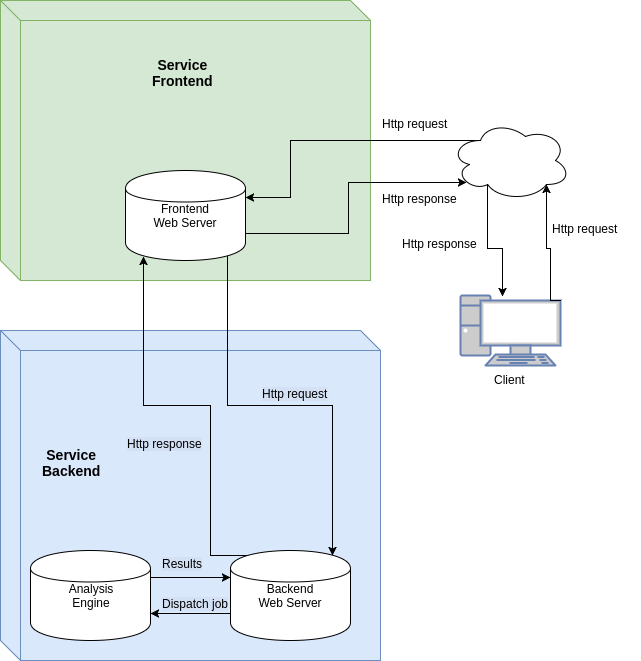
\includegraphics[width=\textwidth]{images/carat-prototype-architecture.png}
	\caption{High level network architecture of the Carat API prototype}
	\label{figure:carat-api-network-prototype}
\end{figure}         

The implementation consists of three main components. These are the front end web server, back end web server and the analysis engine. Figure~\ref{figure:carat-api-network-prototype} shows network level layout of these components and the way these components communicate. When a client accesses the API, the following flow of requests takes place
\begin{enumerate}
	\item Client sends a HTTP request to the front end server. The request may contain parameters that control the way the association rules are generated.
	\item Front end web server sends a HTTP request to the back end web server passing along the parameters from the client.
	\item The back end web server dispatches a job to the analysis engine running on SPARK. Parameters provided by the client are used to control the analysis.
	\item Analysis engine sends generated association rules to the back end web server.
	\item Back end server sends HTTP response containing the generated rules to the front end web server.
	\item Front end server uses the association rules to generate a view for the client.  
\end{enumerate}    
